\mode<presentation>
{
  \usetheme{CambridgeUS}
  \usecolortheme{whale}
  \usecolortheme{lily}

  \setbeamercovered{transparent}
  \usefonttheme[onlymath]{serif}
}

\title[\FirstOrderResponseShortName] 
{\course: \FirstOrderResponseName\license}

\subtitle
{Lecture \FirstOrderResponseNumber} 


\begin{document}

\begin{frame}
  \titlepage
\end{frame}

\mode<article>{
\maketitle
\tableofcontents
}

\section{Pre-requisite Material}
This lecture assumes that the reader is familiar with the following material:
\begin{itemize}
\item Lecture \ImpedanceNumber:~\ImpedanceName
\item Lecture \SolvingDifferentialEquationsAndStabilityNumber:~\SolvingDifferentialEquationsAndStabilityName
\item Lecture \ControlAndStabilityNumber:~\ControlAndStabilityName
\end{itemize}



\section{Introduction}

In the next series of lectures, we want to figure out how we can quickly determine how a system described by a transfer function will respond to typical inputs without having to repeatedly find inverse Laplace Transforms. Consider the following scenarios: 

\subsection{Impulse response}
The suspension system of a car is a control system whose job is to reject disturbances caused by the road. A bump in the road can be considered an impulse. Thus, in designing a suspension system (either active or passive) we are interested in the impulse response of the system between the road position and the car position.

\begin{frame}{Suspension Impulse Response}
\begin{center}
\begin{tikzpicture}
\draw (0,0) node {\includegraphics[width=1.5in]{figures/Porsche_911SC_Slantnose_1982_2.jpg}};
\draw (0,-1.25) node {\begin{minipage}{2in}\tiny\raggedright source: http://upload.wikimedia.org/wikipedia/commons/ 5/5b/Porsche\_911SC\_Slantnose\_1982\_2.jpg\end{minipage}}; 
\draw[very thick] (-2,-0.6) -- (1.5,-.6) -- (2,-.6) arc (180:0:4pt) -- (3,-.6);
\end{tikzpicture}\quad\includegraphics[width=2in]{figures/carimpulseresponse}
\end{center}
\end{frame}

\subsection{Step response}

Many systems are regulated around a set-point. When the system is initially turned on, or the set-point is changed, the input can be considered a step. 

\begin{frame}{Temperature Regulator Response}
\begin{center}
\includegraphics[width=1.5in]{figures/thermostats}\quad\includegraphics[width=2in]{figures/tempstepresponse}
\end{center}
\end{frame}

\subsection{Ramp response}
An example of a system that must track a moving trajectory is a radio telescope that views a celestial object while the earth is moving. In this case, the input can be considered a ramp.

\begin{frame}{Tracking Response}
\begin{center}
\begin{minipage}{1.4in}\includegraphics[width=1.4in]{figures/C-band_Radar-dish_Antenna}\\{\begin{minipage}{1.4in}\tiny\raggedright Source: http://commons.wikimedia.org/wiki/File: C-band\_Radar-dish\_Antenna.jpg\end{minipage}}\end{minipage}\quad\begin{minipage}{2in}\includegraphics[width=2in]{figures/antennarampresponse}\end{minipage}
\end{center}
\end{frame}

%Note to authors: poles/zeros, rational def, and stability def/test were moved to earlier articles

\section{First Order Response}

Let's now start looking at specific types of systems, starting with a first order system with no zeros. We will use the parameterization
\[
G(s)= K\frac{\sigma}{s+\sigma} 
\]
This system has a pole at $s=-\sigma$. The parameter $K$ is called the {\em DC gain}, for reasons that will be clear later.
\subsection{Impulse Response}
If the input is an impulse $r(t)=\delta(t)$, then $R(s)=1$, and the output is given by
\begin{align*}
Y(s) &= G(s)R(s), \\
& =G(s)1,\\
&= K\frac{\sigma}{s+\sigma}.
\end{align*}
So $y(t)$ is simply the inverse Laplace transform of $G(s)$:
\[
y(t) = K\sigma e^{-\sigma t}
\]
\begin{frame}{Impulse Response Plot}
\begin{center}
\includegraphics[height=2in]{figures/impulseresponse}
\begin{definition} 
The {\em time constant} of a first order system is $\tau = \frac{1}{\sigma}$, and is the time for the impulse response - the magnitude of the output signal in response to an impulse input - to decay by 64\%.
\end{definition}
\end{center}
\end{frame}

\subsection{Step Response}
If the input is a step $r(t)=u(t)$, then $R(s)=\frac{1}{s}$, and the output is given by 
\begin{align*}
Y(s) & = G(s)R(s) \\
& = G(s)\frac{1}{s}\\
& = K\frac{\sigma}{s(s+\sigma)}
\end{align*}
The inverse Laplace transform is found using a partial fraction expansion
\[
Y(s) = \frac{K}{s} - \frac{K}{s+\sigma}
\]
so the step response is
\[
y(t) = \left(K - K e^{-\sigma t}\right)u(t)
\]
\begin{frame}{Step Response Settling Time}
\begin{center}
\includegraphics[height=2in]{figures/stepresponse}
\begin{definition} The step response {\em settling time} is the time for the step response - the magnitude of the output signal in response to a step input - to go reach within $1\%$ of the final value, and for a first order system $\ts = \tseqone$ \end{definition}
\end{center}
\end{frame}
The settling time for a first order system can be found by solving
\[
.99K = \left(K - K e^{-\sigma \ts}\right),
\]
or, dividing both sides by $K$ and solving for the exponential term,
\begin{align*}
e^{-\sigma \ts} &= .01\\
-\sigma \ts & = \ln (.01)\\
\ts & = \frac{-\ln(.01)}{\sigma}\\
 & = \frac{4.6}{\sigma}
\end{align*}

\begin{frame}{Step Response Rise Time}
\begin{center}
\includegraphics[height=2in]{figures/stepresponse2}
\begin{definition} The step response {\em rise time} is the time for the step response to go from 10\% to 90\% of its final value, and for a first order system $\tr = \treqone$\end{definition}
\end{center}
\end{frame}
The rise time for a first order system can be found by solving
\begin{align*}
.1K &= \left(K - K e^{-\sigma t_{1}}\right),\\
.9K &= \left(K - K e^{-\sigma t_{2}}\right),\\
\end{align*}
dividing both sides by $K$ and solving for the exponential term,
\begin{align*}
t_{2} & = \frac{-\ln(.1)}{\sigma}\\
t_{1} & = \frac{-\ln(.9)}{\sigma}\\
\tr & = t_{2}-t_{1} =  \frac{2.2}{\sigma}
\end{align*}




\section{Plotting impulse, step, and ramp response in \textsc{Matlab}}
In the following example we will be entering the transfer function
\[
G(s) = \frac{15s+10}{s^{2}+7s+12} = \frac{15(s+\frac{2}{3})}{(s+3)(s+4)}
\]

\subsection{Entering Transfer Functions}
In \textsc{Matlab} you can define variables that are {\em transfer functions}. There are two main commands that we will use, \texttt{zpk} and \texttt{tf}. 
\begin{itemize}
\item Use the command \texttt{zpk} to create a transfer function by specifying the zeros, poles, and gain:
\begin{verbatim}
>> sys=zpk([-2/3],[-3 -4],15)

sys =
 
  15 (s+0.6667)
  -------------
   (s+3) (s+4)
 
Continuous-time zero/pole/gain model.
\end{verbatim}
\item Use the command \texttt{tf} to create a transfer function by specifying the coefficients of the numerator and denominator:
\begin{verbatim}
>> sys=tf([15 10],[1 7 12])

sys =
 
    15 s + 10
  --------------
  s^2 + 7 s + 12
 
Continuous-time transfer function.
\end{verbatim}
\item Once a variable has been defined as a transfer function, you can perform algebraic operations on it (i.e. you can add or multiply two transfer functions together). This gives us another way of entering transfer functions. We can define a variable to be the transfer function $s$, and then use multiplication and division to create the transfer function we want. 

Here we define the variable \texttt{s} to be the transfer function $\frac{s}{1}$.  
\begin{verbatim}
>> s=tf([1 0],1)

s =
 
  s
 
Continuous-time transfer function.
\end{verbatim}
Alternatively, we can use the following form of the \texttt{tf} command
\begin{alltt}
>> s=tf(\T\rule{0pt}{0pt}s\T)
\end{alltt}
\begin{verbatim}
s =
 
  s
 
Continuous-time transfer function.
\end{verbatim}
Once this is done using either method, we use addition, multiplication and division to form the transfer function
\begin{verbatim}
>> sys = (15*s+10)/(s^2+7*s+12)

sys =
 
    15 s + 10
  --------------
  s^2 + 7 s + 12
 
Continuous-time transfer function.
\end{verbatim}
\end{itemize}


\subsection{The \texttt{impulse} and \texttt{step} commands}
Once the transfer function \texttt{sys} is defined, we can plot the impulse and step responses using the commands \texttt{impulse} and \texttt{step}. The resulting plot shows the output signal with the generic y-axis label ``Amplitude'' versus time. \vspace{.1in}\\


\noindent \texttt{>> impulse(sys)}
\begin{center}
\includegraphics[width=3in]{figures/matlabimpulse}
\end{center}
\texttt{>> step(sys)}
\begin{center}
\includegraphics[width=3in]{figures/matlabstep}
\end{center}

There is no ``ramp'' command in \textsc{Matlab}, but since the step response is given by
\[
Y(s)=G(s)\frac{1}{s}
\]
and the ramp response by
\[
Y(s) = G(s)\frac{1}{s^{2}} = \left(G(s)\frac{1}{s}\right)\frac{1}{s}
\]
We can find the ramp response of $G(s)$ by finding the step response of $G(s)\frac{1}{s}$\vspace{.1in}\\
\noindent \texttt{step(sys*tf([1],[1 0]));\\
title('Ramp response')}
\begin{center}
\includegraphics[width=3in]{figures/matlabramp}
\end{center}

You can compare multiple systems by plotting them on the same graph. For example, if we define a second system
using \texttt{>> sys2=tf([1],[1 1]),}
then both step responses are plotted by putting both systems as arguments to the \texttt{step} command\\
\texttt{\\
>> step(sys,sys2)\\
}
\begin{center}
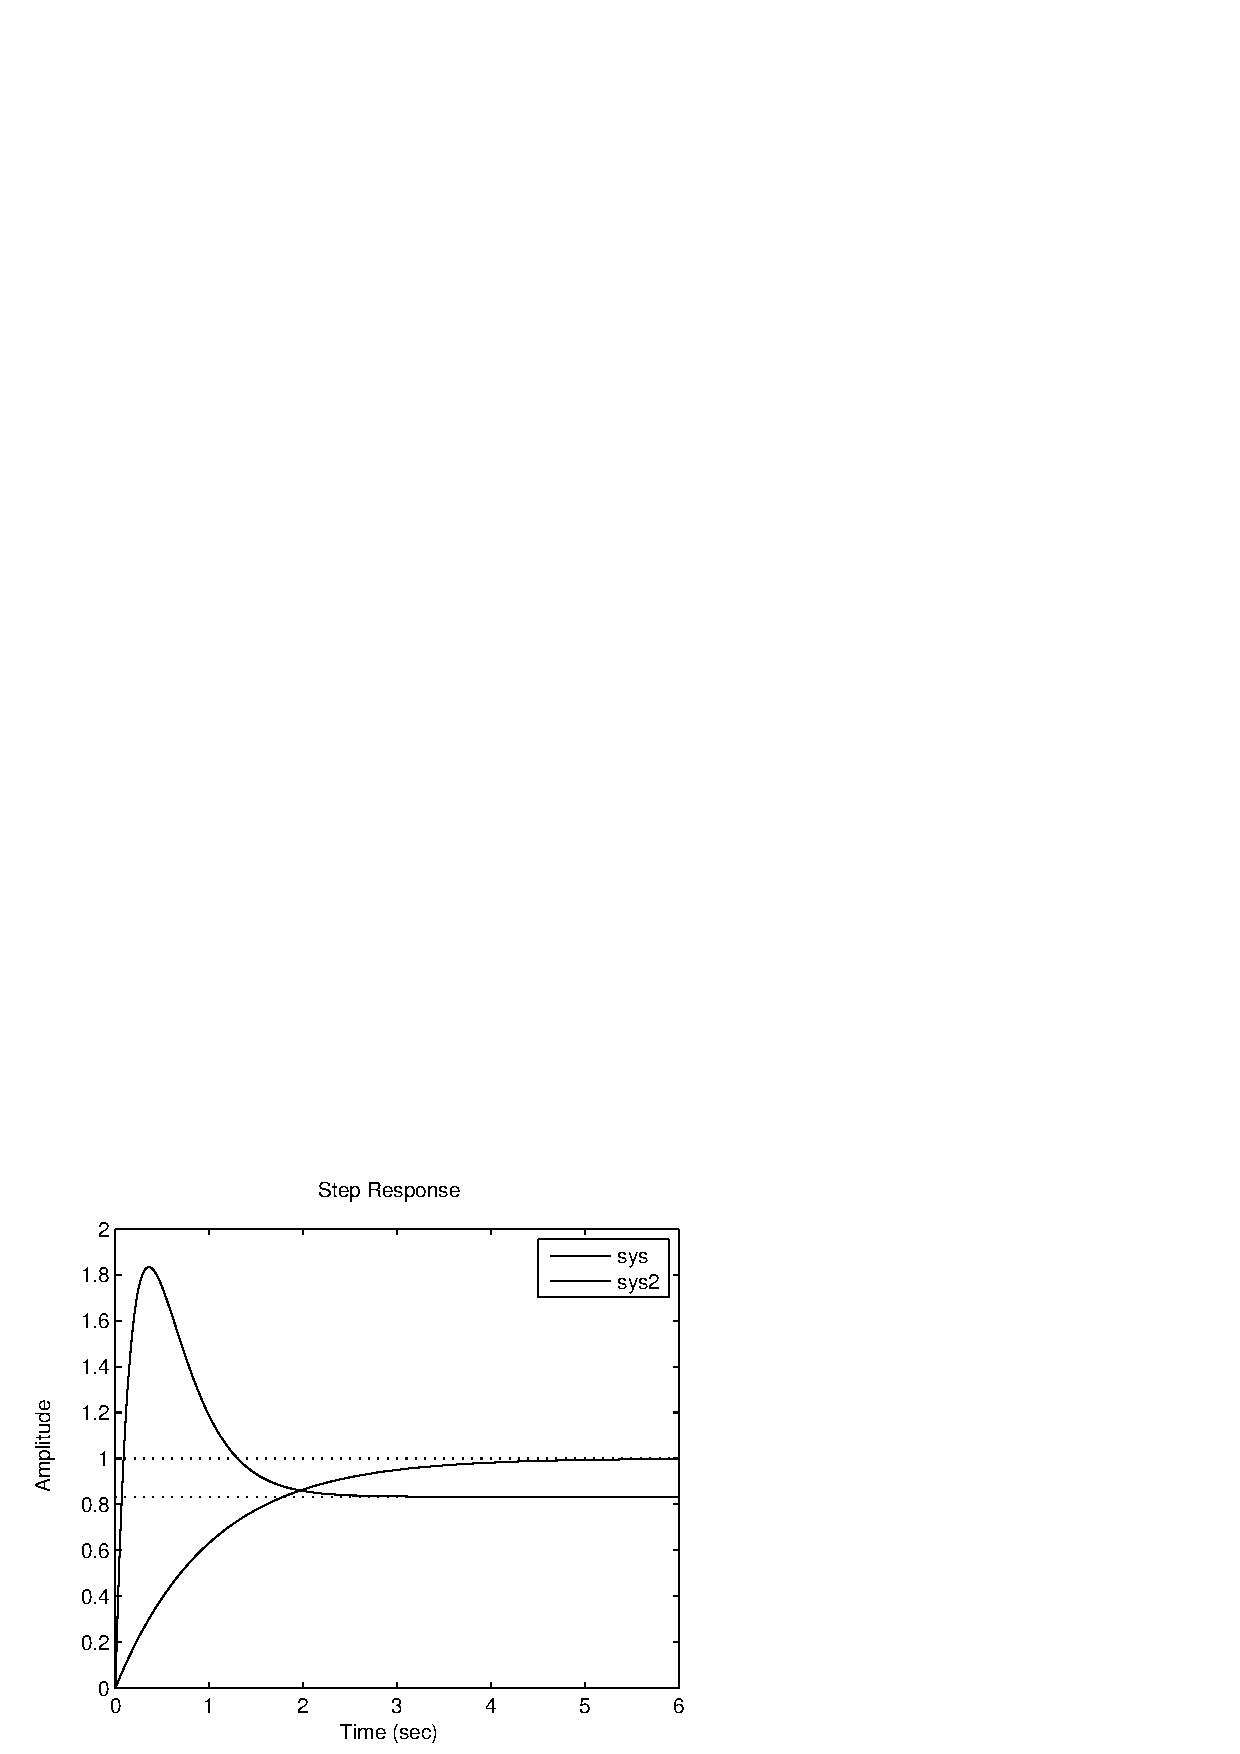
\includegraphics[width=3in]{figures/matlabmultistep}
\end{center}
To get the legend that specifies which response is which, go to the menu on the figure window, and click \texttt{insert->legend}


%In \textsc{Matlab} you can also use the command \texttt{pzplot} to create a pole zero diagram: The pole-zero diagram  in section \ref{sec:polezero} was created using the following commands\vspace{.1in}\\
%\texttt{
%>> sys=tf([1 2 2 0],[1 8 24 32 15])\\
% \\
%Transfer function:\\
%\hspace{1.in}s\^{}3 + 2 s\^{}2 + 2 s\\
%--------------------------------\\
%s\^{}4 + 8 s\^{}3 + 24 s\^{}2 + 32 s + 15\\
%>> pzplot(sys)}


%\subsection{Scilab} 
%To get the step response of the example $G(s)$ given above using Scilab, you would use the following code:\\
%\texttt{s=poly(0,'s')\\
%sys=syslin('c',(15*(s+2/3))/((s+3)*(s+4)))\\
%t=0:.01:2.5\\
%plot2d(t,csim('step',t,sys))}\\
%
%To plot another response on the same plot but with a different line style, define another system as \texttt{sys2} and type\\
%\texttt{plot2d(t,csim('step',t,sys2),style=2)}\\
%
%A legend can be created using \texttt{legend}. For example\\
%\texttt{legend('G1','G2')}
%

\section{Application Example}
A simplified version of the relationship between the wind speed \(u\) and a wind turbine's rotational speed \(\omega = \dot{\theta}\) is given by the transfer function
\begin{equation*}
	\frac{\omega(s)}{u(s)} = \frac{0.5472}{s+0.2867}
\end{equation*}

\begin{center}
	\includegraphics[width=1.5in]{figures/windturbine1.png}
\end{center}

\noindent Based on your understanding of first order system transient response,

\begin{enumerate}[(a)]
	\item Predict how long it will take for $\omega$ to go from 10\% to 90\% of its final value in response to a step change in \(u\).
	\item Predict when \(\omega\) will reach within 1\% of its final value and stay there in response to the same step change in \(u\).
	\item Use Matlab to confirm your answers.
\end{enumerate}

\noindent \textbf{Solutions}

\begin{enumerate}[(a)]
	\item From the transfer function, \(\sigma = 0.2867\) so \(t_s = \frac{2.2}{\sigma} = 7.7 s \).
	\item Similarly, \(t_s = \frac{4.6}{\sigma} = 16s\).\\
	\item We can begin by modeling the transfer function in Matlab and then using the "step" command: \\
\texttt{>> gs  = tf([0.5472],[1 0.2867])}\\
\texttt{>> step(gs)}\\
which results in Figure \ref{fig:response1}, where the final value is 1.91 rpm. Thus, the key points for computing \textbf{rise time} are 0.10(1.91) = 0.19 and 0.90(1.91) = 1.7, and we can either identify these points using the cursor tool \includegraphics[width = .25in]{figures/cursortool.png} or right click \(\rightarrow\) Characteristics \(\rightarrow\) Rise time. The latter option results in a calculation of 7.66 s, which validates our prediction. For \textbf{settling time}, 0.99(1.91) = 1.89, which is marked at 15.9 s, nearly the 16 s predicted.

\end{enumerate}

\begin{center}
\begin{figure}
		\includegraphics[width = 4in]{figures/response1.png}
	\caption{Step response from change in wind speed (m/s) to change in rotor speed (rpm) for simplified wind turbine}
	\label{fig:response1}
\end{figure}
\end{center}


\section{Lecture Highlights}
The primary takeaways from this article include
\begin{enumerate}
\setlength{\itemsep}{5pt}
\setlength{\parskip}{0pt}
\setlength{\parsep}{0pt}
\item Impulse, step, and ramp responses refer to the time-domain behavior of the output signal when the input signal is an impulse, step, or ramp function.
\item We can determine a great deal about the output signal based on the location(s) of the transfer function's pole(s). For this class, when looking at the transient responses of first order systems we will be particularly interested in the rise time and settling time.
\item Matlab can be very useful for the type of analysis used in this lecture. You may find the \texttt{tf}, \texttt{zpk}, \texttt{pole}, \texttt{zero}, \texttt{impulse}, and \texttt{step} commands helpful for checking your work, even if Matlab is not required in a problem statement. (Note: By default, Matlab labels the output signal as ``Amplitude'' on the y axis. You can determine the signal's units from the problem.)
\end{enumerate}


\section{Quiz Yourself}

\subsection{Questions}


\begin{enumerate}
\setlength{\itemsep}{5pt}
\setlength{\parskip}{0pt}
\setlength{\parsep}{0pt}
\item A system is described by the transfer function
\[
\frac{Y(s)}{R(s)} = \frac{5}{s+6}
\]
If $R(s)$ is a unit step, what is the time for the system to settle within 1\% of the final value?\end{enumerate}
\pagebreak

\subsection{Solutions}
\begin{enumerate}
\setlength{\itemsep}{5pt}
\setlength{\parskip}{0pt}
\setlength{\parsep}{0pt}
\item \rule{0pt}{12pt}\\
\begin{center}
\includegraphics[width=5in]{quizfigures/1soln}\\
\end{center}
\end{enumerate}

\section{Resources}

\subsection{Books}

\begin{itemize}
\item Norman S. Nise, {\em Control Systems Engineering}, Wiley
\begin{itemize}
\item 7th edition: Section 4.3 
\end{itemize}
\item Other textbooks tend to focus on second order systems
\end{itemize}

\subsection{Web resources}
There are also some web resources that cover first order response. If you find something useful, or if you find a link that no longer works, please inform your instructor!

\begin{itemize}
\item \url{https://www.youtube.com/watch?v=9itsq4_qNZo}: A 14 minute lecture on step response of first order systems 
\end{itemize}




\end{document}


